\documentclass[11pt, a4paper]{article}
\usepackage[slantfont, boldfont]{xeCJK}
\usepackage{ulem}
\usepackage{amsmath}
\usepackage{booktabs}
\usepackage{colortbl}
\usepackage{fancyvrb}
\usepackage{multirow}
\usepackage[top = 1.0in, bottom = 1.0in, left = 1.0in, right = 1.0in]{geometry}

\setCJKmainfont{SimSun}
\setCJKmonofont{SimSun}

\setlength{\parskip}{0.5\baselineskip}
\setlength{\parindent}{2em}

\title{Codeforces. Counting Skyscrapers}
\author{VFleaKing}

\begin{document}
\maketitle

\section*{题目描述}
大街上建好了一排摩天大楼。摩天大楼的数量是在 $2$ 到 $314!$($314$的阶乘,一个非常大的数)中均匀随机选择的。每座摩天大楼的高度(即楼层数)是被独立地随机选择的:对于每个正整数 $i$,楼层数为 $i$ 的概率为 $2^{-i}$。如果一座摩天大楼有 $i$ 层,那么它的楼层被编号为 $0$ 到 $i - 1$。

为了加快中转运输的效率,摩天大楼间修建了一些滑索。一座摩天大楼的第 $i$ 层和另一座摩天大楼的第 $i$ 层之间有滑索当且仅当两楼之间没有摩天大楼有第 $i$ 层。

Alice和Bob想数一数有多少座摩天大楼。

Alice是个严谨认真的人,她想知道摩天大楼数量的准确值。于是她把计数器初始化为 $1$,从最左边的摩天大楼开始往右走,每次走到一个摩天大楼就把计数器加上 $1$,直到她到达最右边的摩天大楼。

Bob很没耐心,他想尽快完成任务。于是他把计数器初始化为 $1$,从最左边的摩天大楼开始利用滑索从一座摩天大楼滑到另一座。因为恐高,每次他会忽略那些高度(即所在楼层编号)大于 $h$ 的滑索,然后在剩下的往右滑的滑索中选一个最高的。由于Bob使用滑索时滑得太快以至于他无法数清经过了多少座摩天大楼,所以他直接将计数器加上 $2^i$,其中 $i$ 是他当前所在的楼层编号。他会一直持续这个过程直到他到达最右边的摩天大楼。

考虑下面这个例子。这里有 $6$ 栋楼,高度从左到右分别为 $1, 4, 3, 4, 1, 2$,并且 $h = 2$。Alice的计数器初始为 $1$ 然后加了 $5$ 次 $1$ 得到结果是 $6$。Bob的计数器初始为 $1$ 然后依次加上 $1, 4, 4, 2$ 得到结果 $12$。注意Bob会忽略最高的那个滑索因为他恐高($h = 2$)。

\begin{figure}[h]
\centering
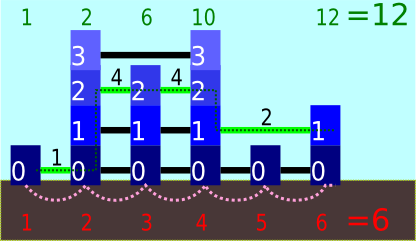
\includegraphics[scale=0.7]{sample.png}
\end{figure}

Bob的计数器的值在这张图的最上面,Alice的计数器的值在这张图最下面。图中的横线是滑索,绿色虚线表示Bob的路线,粉色虚线表示Alice的路线。摩天大楼上的数字是楼层编号,Bob经过的滑索上的数字是他计数器在此处的增加量。

当Alice和Bob到达最右边的摩天大楼时,他们会比较计数器的值。现在给出Alice的计数器的值或者Bob的计数器的值,请你求出另一人的计数器的值的期望。

\section*{输入格式}
第一行是一个名字,为``\texttt{Alice}''或``\texttt{Bob}''。

第二行包括两个整数 $n$ 和 $h$ $(n \geq 2, h \geq 0)$。如果名字是``\texttt{Alice}'',那么 $n$ 表示Alice到达最右边的摩天大楼时她的计数器的值,否则 $n$ 表示Bob到达最右边的摩天大楼时他的计数器的值。$h$ 表示Bob愿意使用的滑索的最高楼层编号。

\section*{输出格式}
如果给出的是Bob的计数器的值,输出一个实数表示Alice的计数器的期望值;如果给出的是Alice的计数器的值,输出一个实数表示Bob的计数器的期望值。

你的答案被认为是正确的当且仅当你的答案与标准答案的绝对误差或相对误差不超过 $10^{-9}$。

\section*{样例1}
\begin{Verbatim}[frame=single, label=input]
Alice
3 1

\end{Verbatim}

\begin{Verbatim}[frame=single, label=output]
3.500000000

\end{Verbatim}
Bob的计数器有 $62.5\%$ 的概率是 $3$, 有 $25\%$ 的概率是 $4$, 有 $12.5\%$ 的概率是 $5$。

\section*{样例2}
\begin{Verbatim}[frame=single, label=input]
Bob
2 30

\end{Verbatim}

\begin{Verbatim}[frame=single, label=output]
2.000000000

\end{Verbatim}

\section*{样例3}
\begin{Verbatim}[frame=single, label=input]
Alice
2572 10

\end{Verbatim}

\begin{Verbatim}[frame=single, label=output]
3439.031415943

\end{Verbatim}

\section*{数据范围}
\begin{center}
\begin{tabular}{|c|p{70pt}|p{70pt}|p{70pt}|}
    \hline
    \#    & who   & $n$  & $h$ \\
    \hline
    1    & \multirow{10}{*}{Alice} & $\leq 30000$                  & $= 0$                      \\
    \cline{1-1}\cline{3-4}
    2    &                         & \multirow{2}{*}{$\leq 15$}    & \multirow{2}{*}{$= 1$}     \\
    \cline{1-1}
    3    &                         &                               &                            \\
    \cline{1-1}\cline{3-4}
    4    &                         & \multirow{1}{*}{$\leq 50$}    & \multirow{1}{*}{$\leq 30$} \\
    \cline{1-1}\cline{3-4}
    5    &                         & \multirow{1}{*}{$\leq 100$}   & \multirow{1}{*}{$\leq 30$} \\
    \cline{1-1}\cline{3-4}
    6    &                         & \multirow{2}{*}{$\leq 1000$}  & \multirow{2}{*}{$\leq 30$} \\
    \cline{1-1}
    7    &                         &                               &                            \\
    \cline{1-1}\cline{3-4}
    8    &                         & \multirow{3}{*}{$\leq 30000$} & \multirow{3}{*}{$\leq 30$} \\
    \cline{1-1}
    9    &                         &                               &                            \\
    \cline{1-1}
    10   &                         &                               &                            \\
    \hline
    11   & \multirow{10}{*}{Bob}   & $\leq 30000$                  & $= 0$                      \\
    \cline{1-1}\cline{3-4}
    12   &                         & \multirow{2}{*}{$\leq 15$}    & \multirow{2}{*}{$= 1$}     \\
    \cline{1-1}
    13   &                         &                               &                            \\
    \cline{1-1}\cline{3-4}
    14   &                         & \multirow{1}{*}{$\leq 50$}    & \multirow{1}{*}{$\leq 30$} \\
    \cline{1-1}\cline{3-4}
    15   &                         & \multirow{1}{*}{$\leq 100$}   & \multirow{1}{*}{$\leq 30$} \\
    \cline{1-1}\cline{3-4}
    16   &                         & \multirow{2}{*}{$\leq 1000$}  & \multirow{2}{*}{$\leq 30$} \\
    \cline{1-1}
    17   &                         &                               &                            \\
    \cline{1-1}\cline{3-4}
    18   &                         & \multirow{3}{*}{$\leq 30000$} & \multirow{3}{*}{$\leq 30$} \\
    \cline{1-1}
    19   &                         &                               &                            \\
    \cline{1-1}
    20   &                         &                               &                            \\
    \hline
\end{tabular}
\end{center}

时间限制:$1\text{s}$

空间限制:$256\text{MB}$

\section*{题解}
用 $Pr(P)$ 表示表达式 $P$ 成立的概率。

用 $EX$ 表示随机变量 $X$ 的期望值。
\subsection*{简单的分析}
这个问题分为两部分:Alice部分和Bob部分。

记题目中的 $h$ 为 $h_m$。

记Alice的计数器的值为随机变量 $L_A$, Bob的计数器的值为随机变量 $L_B$。

这个问题相当于说摩天大楼高度在$0$到$h_m$之间(为了方便我们重新定义摩天大楼的高度为最高楼层的编号。高度为 $h$ 即有 $h + 1$ 层),且:
\begin{equation}
Pr(H = h) =
	\begin{cases}
	2^{-h - 1}   & \mbox{$0 \leq h < h_m$}\\
	2^{-h_m} & \mbox{$h = h_m$}
	\end{cases}
\end{equation}
其中随机变量 $H$ 表示一座摩天大楼的高度。

Alice部分:$E(L_B | L_A = n)$。(共 $50$ 分)

Bob部分:$E(L_A | L_B = n)$。(共 $50$ 分)

\subsection*{算法一}
对于1, 11号测试点,$h_m = 0$,所以只有高度为 $0$ 的大楼,Bob一定会老老实实地走完全程。

于是答案为 $E(L_A | L_B = n) = n, E(L_B | L_A = n) = n$。

可以通过1, 11号测试点获得10分。

\subsection*{算法二}
对于2, 3号测试点,$h_m = 1$,所以高度要么为 $0$ 要么为 $1$,除此之外 $n$ 又特别小。

可以考虑 $O(2^n)$ 暴力枚举所有情况然后算出对应的 $L_B$ 取值,从而得出 $L_B$ 的概率分布算出期望。总时间复杂度 $O(n 2^n)$。

可以通过2, 3号测试点获得10分。

\subsection*{算法三}
考虑Bob部分。

我们称Bob走到过的楼为接点楼。(不包括在空中滑过的楼)

如果我已知所有接点楼的高度,那么滑索的高度和Bob计数器值都好求。但是,此时的 $EL_A$ 是多少?

我们可以对于每个滑索单独考虑经过的摩天大楼的期望数量(不包括左端点,包括右端点),由于摩天大楼的数量上限为 $314!$ 足够大以至于可以视为无穷大,于是可以认为每根滑索经过的摩天大楼的数量这个随机变量是相互独立的。由于期望的线性性,我们可以单独计算每根滑索经过的摩天大楼的期望数量再加上Alice计数器初始值 $1$ 得到 $EL_A$。

考虑一根Bob走过的且高度为 $h_t$ 的滑索,那么中间的摩天大楼的高度一定要满足高度小于 $h_t$。

设滑索经过摩天大楼数(不包括左端点,包括右端点)为随机变量 $L$,设条件 $P_L$ 为中间的 $L - 1$ 个摩天大楼的高度都小于 $h_t$。则:
\begin{equation}
Pr(L = l | P_L) = \frac{Pr(P_L \cap L = l)}{Pr(P_L)} = \frac{Pr(L = l) Pr(P_L | L = l)}{\sum_{k \geq 1}{Pr(L = k) Pr(P_L | L = k)}}
\end{equation}
由于摩天大楼数量是均匀随机选取的,所以:
\begin{eqnarray}
Pr(L = l | P_L) & = & \frac{Pr(P_L | L = l)}{\sum_{k \geq 1}{Pr(P_L | L = k)}}\\
                & = & \frac{Pr(H < h_t)^{l - 1}}{\sum_{k \geq 1}{Pr(H < h_t)^{k - 1}}}\\
                & = & \frac{(1 - 2^{-h_t})^{l - 1}}{\sum_{k \geq 1}{(1 - 2^{-h_t})^{k - 1}}}\\
                & = & 2^{-h_t}(1 - 2^{-h_t})^{l - 1}
\end{eqnarray}
于是可以求出期望:
\begin{eqnarray}
E(L | P_L) & = & \sum_{l \geq 1}{Pr(L \geq l | P_L)}\\
           & = & \sum_{l \geq 1}{(1 - 2^{-h_t})^{l - 1}}\\
           & = & \frac{1}{2^{-h_t}}\\
           & = & 2^{h_t}
\end{eqnarray}

再来看滑一次之后Bob的计数器的变化:增加了$2^{h_t}$。

我们惊奇的发现,Bob的估计恰好和期望值相等。

所以结论是:$E(L_A | L_B = n) = n$。

可以通过11号到20号测试点获得50分。

后50分设置的其它部分分档次是给各种暴力、近似算法、打表准备的。当然我认为很大程度上得分的前提都取决于求出$E(L | P_L)$,没有观察到这个与Bob计数器一致的话会陷入求每一种``已知接点楼的高度''的方案出现的概率的僵局,需要更多的数学计算。如果不幸陷入却得到了解法但无法得全分,还是可以得到我设置的各种部分分的。

\subsection*{算法三}
$E(L_A | L_B = n)$ 的值是简单的$n$,但是反之 $E(L_B | L_A = n)$ 却不尽然。

观察Bob的行走路线,一定是先往右,高度逐渐升高,到达最高的摩天大楼后再往右,高度逐渐降低。

考虑dp。记最左边的摩天大楼的高度为随机变量 $H_0$,设条件 $D_i$ 为从左往右数第$i$个摩天大楼是它右边的楼及它自己中最高的(从 $1$ 开始编号)。转移时考虑最左边的Bob使用的滑索,设最左边的Bob使用的滑索经过的摩天大楼数(不包括左端点,包括右端点)为随机变量$L$,高度为随机变量$H_p$。则:
\begin{multline}
E(L_B | L_A = n, H_0 = h_0) = \\
\sum_{l = 1}^{n - 1}\sum_{h_r = 0}^{h_0 - 1}{Pr(L = l, H_p = h_r, D_{l + 1} | L_A = n, H_0 = h_0) \left(2^{h_r} + E(L_B | L_A = n - l, H_0 = h_r, D_1)\right)}\\
+ \sum_{l = 1}^{n - 1}\sum_{h_r = h_0}^{h_m}{Pr(L = l, H_p = h_r | L_A = n, H_0 = h_0) \left(2^{h_0} + E(L_B | L_A = n - l, H_0 = h_r) \right)}
\end{multline}
注意到:
\begin{equation}
Pr(L = l, H_p = h_r | L_A = n, H_0 = h_0) = Pr(H < h_r)^{l - 1} Pr(H = h_r)
\end{equation}
\begin{equation}
Pr(L = l, H_p = h_r, D_{l + 1} | L_A = n, H_0 = h_0) = Pr(H < h_r)^{l - 1} Pr(H = h_r) Pr(H \leq h_r)^{n - l - 1}
\end{equation}
于是问题只剩下 $E(L_B | L_A = n - l, H_0 = h_r, D_1)$。这个可以如法炮制:
\begin{multline}
E(L_B | L_A = n, H_0 = h_r, D_1) = \\
\sum_{l = 1}^{n - 1}\sum_{h_r = 0}^{h_0}{Pr(L = l, H_p = h_r, D_{l + 1} | L_A = n, H_0 = h_0, D_1) \left(2^{h_r} + E(L_B | L_A = n - l, H_0 = h_r, D_1)\right)}
\end{multline}
注意到:
\begin{multline}
Pr(L = l, H_p = h_r, D_{l + 1} | L_A = n, H_0 = h_0, D_1) = \\
Pr(H < h_r | H \leq h_0)^{l - 1} Pr(H = h_r | H \leq h_0) Pr(H \leq h_r | H \leq h_0)^{n - l - 1}
\end{multline}
也即:
\begin{multline}
Pr(L = l, H_p = h_r, D_{l + 1} | L_A = n, H_0 = h_0, D_1) = \\
Pr(H < h_r)^{l - 1} Pr(H = h_r) Pr(H \leq h_r)^{n - l - 1} / Pr(H \leq h_0)^{n - 1}
\end{multline}

于是可以进行递推求解。直接暴力递推的复杂度为 $O(n^2h^2)$。

可以通过2,3,4,5号测试点获得20分。若与算法一相结合可以获得30分。

4号测试点是为该算法实现得极其糟糕或者由于某些原因在大数据情况下会精度误差偏大的选手准备的。

\subsection*{算法四}
可以在算法三基础上利用前缀和进行优化。复杂度降为 $O(n h^2)$。见 \texttt{E\_dp.cpp}。

可以通过1号到7号测试点获得35分。

\subsection*{算法五}
可以发现,算法三和算法四实在不是一个优美的算法,再优化下去存在难度。当事情变得越来越复杂的时候,有可能是我们处理的方式不对。

让我们考虑 $h_m = 1$,由算法一知 $E(L_A | L_B = n) = n$。

再考虑 $h_m = 2$,仔细想想我们真的需要像算法二那样暴力枚举所有情况才能得到答案吗?事情并非如此。其实很容易推出一个简洁的表达式。

我们的思路是:逐步增加 $h_m$。每次增加 $h_m$ 时,相当于说原来高度为 $h_m$ 的摩天大楼中有一些升高到了 $h_m + 1$,我们考虑这件事情对$E(L_A | L_B = n)$的影响。

由于期望的线性性,我们可以考虑每两点之间的滑索对期望的影响。

假设现在 $h_m$ 从 $h - 1$ 增加到了 $h$,我们考虑一根新出现的高度为 $h$ 的滑索。该滑索下面会有若干条高度为$h - 1$的滑索,这些是当$h_m = h - 1$时Bob的行走路线。而当$h_m = h$时,Bob放弃了这些滑索。所以一根新出现的高度为 $h$ 的滑索对Bob计数器的期望的贡献为:
该滑索对Bob的计数器的期望的影响为:
\begin{equation}
Pr(\text{该滑索存在}) \times \left( E(\text{经过该滑索带来的增加量}) - E(\text{Bob放弃下面的滑索带来的损失}) \right)
\end{equation}
假设这根滑索经过了$l$座摩天大楼(不包括左端点,包括右端点),那么该滑索存在的概率为:
\begin{eqnarray}
Pr(\text{该滑索存在}) & = & Pr(H = h) Pr(H < h)^{l - 1} Pr(H = h)\\
& = & 2^{-2h} (1 - 2^{-h})^{l - 1}
\end{eqnarray}
由于该滑索高度为$h$,所以必有:
\begin{equation}
E(\text{经过该滑索带来的增加量}) = 2^h
\end{equation}
接下来考虑损失。即要求下方的滑索的期望条数,也即中间高度为$h - 1$的摩天大楼的期望数量加$1$(右端点肯定高度$\geq h - 1$):
\begin{eqnarray}
E(\text{Bob放弃下面的滑索带来的损失}) & = & \left((l - 1) \cdot Pr(H = h - 1 | H < h) + 1 \right) \cdot 2^{h - 1}\\
& = & \left((l - 1) \cdot \frac{2^{-h}}{1 - 2^{-h}} + 1 \right) \cdot 2^{h - 1}\\
& = & \left(\frac{l - 1}{2^h - 1} + 1 \right) \cdot 2^{h - 1}
\end{eqnarray}
考虑到经过$l$座摩天大楼的滑索一共有 $n - l$ 个可能的位置,于是我们得到当$h_m$从$h - 1$变为$h$时的期望变化量为:
\begin{equation}
\sum_{l = 1}^{n - 1}{(n - l) 2^{-2h} (1 - 2^{-h})^{l - 1} \left(2^h - \left(\frac{l - 1}{2^h - 1} + 1 \right) \cdot 2^{h - 1} \right)}
\end{equation}
化简得:
\begin{equation}
\sum_{l = 1}^{n - 1}{(n - l) 2^{-h} (1 - 2^{-h})^{l - 1} \left(\frac{1}{2} - \frac{1}{2} \cdot \frac{l - 1}{2^h - 1} \right)}
\end{equation}
由于初始$h_m = 0$时 $E(L_A | L_B = n) = n$,故对于任一$h_m$有:
\begin{equation}
E(L_A | L_B = n) = n + \sum_{h = 1}^{h_m}{\sum_{l = 1}^{n - 1}{(n - l) 2^{-h} (1 - 2^{-h})^{l - 1} \left(\frac{1}{2} - \frac{1}{2} \cdot \frac{l - 1}{2^h - 1} \right)}}
\end{equation}

于是我们得到了一个时间复杂度为 $O(nh)$ 的算法。

可以通过1号到10号测试点获得50分。

\subsection*{算法六}
结合算法三和算法五就能通过所有测试点获得100分。完美解决此题。

\end{document}
